\documentclass{article}
\usepackage[utf8]{inputenc}

\title{Tarea 4 metodos computacionales}
\author{Maria Camila Garcia 20151657 }
\date{19 de Noviembre 2018}

\usepackage{natbib}
\usepackage{graphicx}

\begin{document}

\maketitle
\section{ODE}
La siguiente gráfica es para el proyectil lanzado con un ángulo de 45 grados, la distancia máxima obtenida es de x=4.17 metros y se tiene una altura máxima cercana a y=3.00 metros. No se tiene una parábola perfecta ya que la gravedad y la resistencia del aire forman el tiro parabólico y además como debido a la fricción tanto en x como en y se curva el movimiento.

\begin{center}
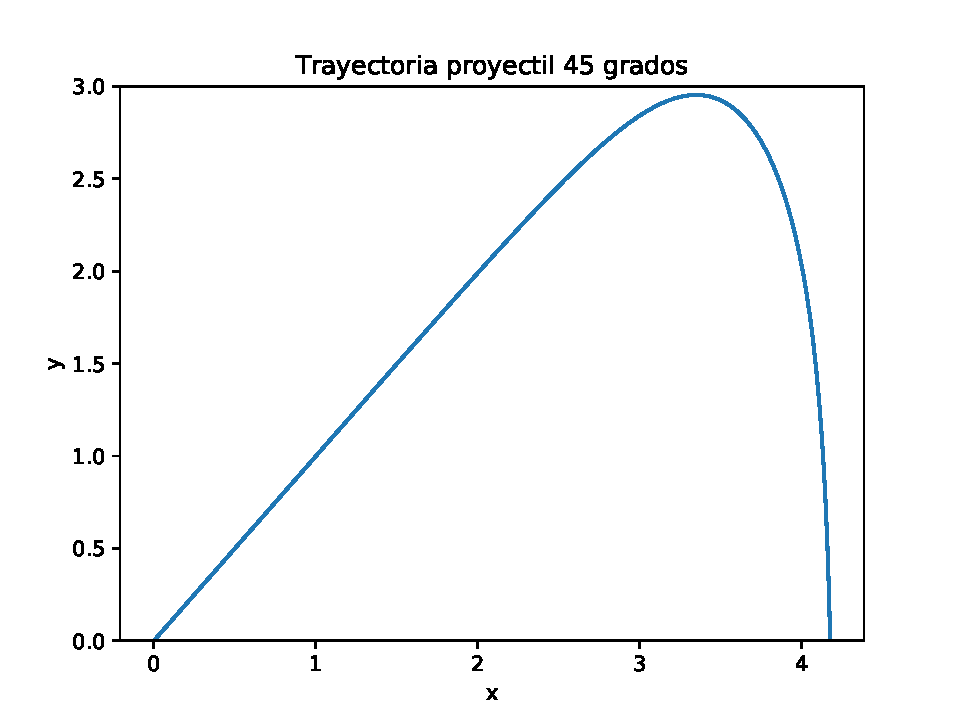
\includegraphics[width=13cm, height=7cm]{ODE1.pdf}\\
\small{Figura 1: Gráfica de trayectoria del proyectil para 45 grados.}
\end{center}

Ahora se ve la gráfica para el proyectil lanzado con diferentes ángulos y se puede observar que para los ángulos más pequeños hay mayores distancias recorridas y para los mas grandes se recorre menos distancia, como en el punto anterior se ve que el tiro no es perfectamente parabólico.
\begin{center}
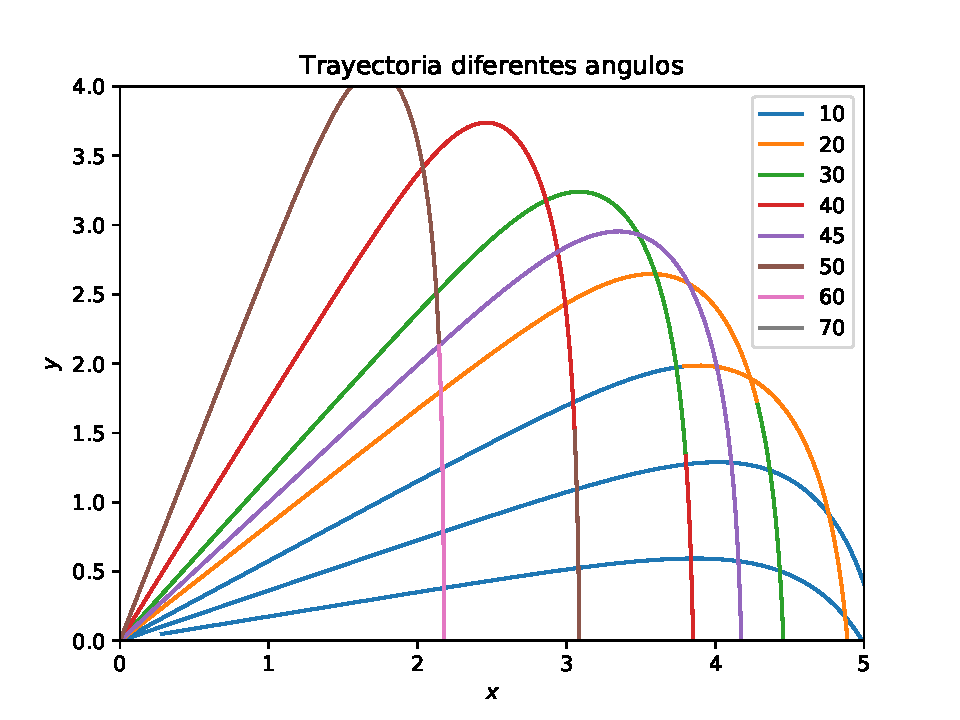
\includegraphics[width=13cm, height=7cm]{ODE2.pdf}\\
\small{Figura 2: Gráfica de trayectoria del proyectil para  los demás ángulos.}
\end{center}

\section{PDE}
Las siguientes gráficas de difusión representan un sistema de una piedra caliza que inicialmente se encuentra a temperatura 10 grados y se pone en contacto con una varilla que esta a 100 grados perpendicular en el centro de la misma, y se observa el cambio de la temperatura de la roca conforme avanza el tiempo. 

\subsection{Extremos fijos}
Para este primer caso podemos ver que se tiene una temperatura de 10 grados en los extremos de todas las gráficas.\\
Para la condición inicial podemos ver que se tiene la temperatura de la roca a 10 grados y la de la varilla a 100.
\begin{center}
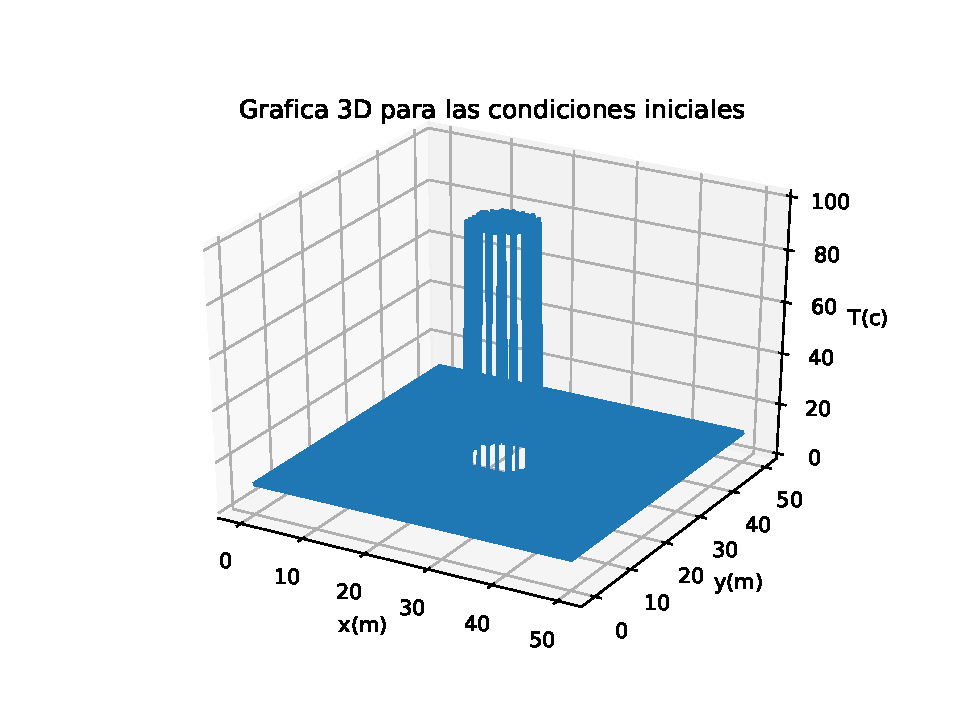
\includegraphics[width=13cm, height=7cm]{3DCondIni.pdf}\\
\small{Figura 3: Condiciones iniciales, extremos fijos.}
\end{center}

Las siguientes dos gráficas muestran el cambio de la temperatura respecto al tiempo, se puede observar un aumento general de temperatura de la roca . 
\begin{center}
\includegraphics[width=13cm, height=7cm]{3Dintermedios1.pdf}\\
\small{Figura 4: Extremos fijos, caso 1.}
\end{center}

\begin{center}
\includegraphics[width=13cm, height=7cm]{3Dintermedios2.pdf}\\
\small{Figura 5: Extremos fijos, caso 2.}
\end{center}

La siguiente gráfica muestra el punto estable al que se llega en el proceso, se llego al punto en el que no aumenta ni disminuye la temperatura.


\begin{center}
\includegraphics[width=13cm, height=7cm]{3Dintermerdios3.pdf}\\
\small{Figura 6: Extremos fijos, caso 3.}
\end{center}

\subsection{Extremos libres}

Para extremos libres las partículas de los extremos se comportan libremente. En la sieguiente gráfica se ven las condiciones libres.

\begin{center}
\includegraphics[width=13cm, height=7cm]{Libres13D.pdf}\\
\small{Figura 7: Condiciones iniciales, extremos libres.}
\end{center}

Las siguientes figuras muestran el movimiento total, como los extremos no son fijos se va aumentando la temperatura hasta encontrar el equilibrio.
\begin{center}
\includegraphics[width=13cm, height=7cm]{primerolibres.pdf}\\
\small{Figura 8: Extremos libres, caso 1.}
\end{center}

\begin{center}
\includegraphics[width=13cm, height=7cm]{segundolibres.pdf}\\
\small{Figura 9: Extremos libres, caso 2.}
\end{center}

Finalmente, es posible ver como llega al equilibrio.
\begin{center}
\includegraphics[width=13cm, height=7cm]{tercerolibres.pdf}\\
\small{Figura 10: Extremos libres, caso 3.}
\end{center}

\subsection{P. Periódica}

Para los extremos periódicos se considera la placa como conectada a otras cuatro placas en sus extremos, esta situacion determina el comportamiento de las fronteras de nuestra placa.

\begin{center}
\includegraphics[width=13cm, height=7cm]{3DPeriodicasIniciales.pdf}\\
\small{Figura 11: Condiciones iniciales, p. periodica.}
\end{center}

En general, todas las gráficas son bastantes similares a las de extremos libres gracias a la simetria del sistema.
\begin{center}
\includegraphics[width=13cm, height=7cm]{primeroperiodica.pdf}\\
\small{Figura 12: P.periódica, caso 1.}
\end{center}

\begin{center}
\includegraphics[width=13cm, height=7cm]{segundoperiodica.pdf}\\
\small{Figura 13: P.periódica, caso 2.}
\end{center}

En esta última gráfica se puede ver como la temperatura aumenta y cuando se llega al valor de equilibrio toda la placa se encuentra en 100 grados.

\begin{center}
\includegraphics[width=13cm, height=7cm]{terceraperiodica.pdf}\\
\small{Figura 14: P.periódica, caso 3.}
\end{center}

\end{document}
